\documentclass{notes}

\theoremstyle{plain}
\newtheorem{theorem}{Theorem}[chapter]
\newtheorem*{definition}{Definition}
\newtheorem*{corollary}{Corollary}
\newtheorem*{example}{Example}
\newtheorem{lemma}{Lemma}[chapter]
\newtheorem*{notes}{Notes}
\newtheorem*{proposition}{Proposition}
\newtheorem*{note}{Note}
\newtheorem*{notation}{Notation}

\newcommand{\Q}{\mathbb{Q}}
\newcommand{\nequiv}{\not\equiv}
\newcommand{\rel}{\mathrel{\mathcal{R}}}
\newcommand{\relset}{\mathcal{R}}
\DeclareMathOperator{\hcf}{hcf}
\DeclareMathOperator{\sym}{sym}
\DeclareMathOperator{\sign}{sign}

\begin{document}
\frontmatter
\title{Discrete Mathematics}
\lecturer{Dr.~J.~Saxl}
\maintainer{Paul Metcalfe}
\date{Mich\ae lmas 1995} \maketitle

\thispagestyle{empty}
\noindent\verb$Revision: 2.4 $\hfill\\
\noindent\verb$Date: 2001/11/01 09:42:47 $\hfill

\vspace{1.5in}

The following people have maintained these notes.

\begin{center}
\begin{tabular}{ r  l}
-- date & Paul Metcalfe
\end{tabular}
\end{center}

\tableofcontents

\chapter{Introduction}

These notes are based on the course ``Discrete Mathematics''
given by Dr.~J.~Saxl in Cambridge in the Mich\ae lmas Term 1995.  These
typeset notes are totally unconnected with Dr.~Saxl.

\alsoavailable
\archimcopyright

\mainmatter

\chapter{Integers}

\begin{notation}
The ``natural numbers'', which we will denote by $\N$, are
\[
\{ 1,2,3,\dots \}.
\]  The integers $\Z$ are 
\[\{ \dots, -2, -1, 0, 1, 2, \dots \}.
\]  We will also use the non-negative integers, denoted either by
$\N_0$ or $\Z_+$, which is $\N \cup \{ 0 \}$.  There are also the rational
numbers $\Q$ and the real numbers $\R$.

Given a set $S$, we write $x \in S$ if $x$ belongs to $S$, and
$x \notin S$ otherwise.
\end{notation}

There are operations $+$ and $\cdot$ on $\Z$.  They have certain
``nice'' properties which we will take for granted.  There is also
``ordering''.  $\N$ is said to be ``well-ordered'', which means that
every non-empty subset of $\N$ has a least element.  The principle
of induction follows from well-ordering.

\begin{proposition}[Principle of Induction]
Let $P(n)$ be a statement about $n$ for each $n \in \N$.  Suppose
$P(1)$ is true and $P(k)$ true implies that $P(k+1)$ is true for each
$k \in \N$.  Then $P$ is true for all $n$.
\end{proposition}

\begin{proof}
Suppose $P$ is not true for all $n$.  Then consider the subset $S$ of
$\N$ of all numbers $k$ for which $P$ is false. Then $S$ has a least
element $l$.  We know that $P(l-1)$ is true (since $l > 1$), so that
$P(l)$ must also be true.  This is a contradiction and $P$ holds for
all $n$.
\end{proof}

\section{Division}

Given two integers $a$, $b \in \Z$, we say that $a$ divides $b$
(and write $a \mid b$) if $a \neq 0$ and $b = a \cdot q$ for some $q \in \Z$
($a$ is a divisor of $b$). $a$ is a \emph{proper divisor} of $b$ if
$a$ is not $\pm 1$ or $\pm b$.

\begin{note}
If $a \mid b$ and $b \mid c$ then $a \mid c$, for if $b = q_1 a$
and $c = q_2 b$ for $q_1$, $q_2 \in \Z$ then $c = (q_1 \cdot q_2) a$.
If $d \mid a$ and $d \mid b$ then $d \mid ax + by$.  The proof of this is
left as an exercise.
\end{note}

\section{The division algorithm}

\begin{lemma}\label{L:divalg}
Given $a$, $b \in \N$ there exist unique integers $q$, $r \in \N$ with
$a = q b + r$, $0 \le r < b$.
\end{lemma}

\begin{proof}
Take $q$ the largest possible such that $q b \le a$ and put $r = a - q b$.
Then $0 \le r < b$ since $a - qb \ge 0$ but $(q+1) b \ge a$.  Now suppose
that $a = q_1 b + r$ with $q_1$, $r_1 \in \N$ and $0 \le r_1 < b$.  Then
$0 = (q - q_1) b + (r - r_1)$ and $b \mid r - r_1$.  But
$-b < r - r_1 < b$ so that $r = r_1$ and hence $q = q_1$.
\end{proof}

It is clear that $b \mid a$ iff $r = 0$ in the above.

\begin{definition}
Given $a$, $b \in \N$ then $d \in \N$ is the highest common factor
(greatest common divisor) of $a$ and $b$ if:
\begin{enumerate}
\item $d \mid a$ and $d \mid b$,
\item if $d' \mid a$ and $d' \mid b$ then $d' \mid d$ ($d' \in \N$).
\end{enumerate}
\end{definition}

The highest common factor (henceforth hcf) of $a$ and $b$ is 
written $(a,b)$ or $\hcf (a,b)$.

The hcf is obviously unique --- if $c$ and $c'$ are both hcf's then
they both divide each other and are therefore equal.

\begin{theorem}[Existance of hcf]\label{T:exthcf}
For $a$, $b \in \N$ $\hcf (a,b)$ exists.  Moreover there exist integers
$x$ and $y$ such that $(a,b) = a x + b y$.
\end{theorem}

\begin{proof}
Consider the set $I = \{ a x + b y : x,y \in \Z \text{ and }
a x + b y > 0 \}$.  Then $I \neq \emptyset$ so let $d$ be the least
member of $I$.  Now $\exists x_0, y_0$ such that
$ d = a x_0 + b y_0$, so that if $d' \mid a$ and $d' \mid b$ then
$d' \mid d$.

Now write $a = q d + r$ with $q$, $r \in \N_0$, $0 \le r < d$.  We
have $r = a - qd = a ( 1 - q x_0) + b( -q y_0)$.  So $r = 0$, as otherwise
$r \in I$: contrary to $d$ minimal.  Similiarly, $d \mid b$ and thus
$d$ is the hcf of $a$ and $b$.
\end{proof}

\begin{lemma}\label{L:toeuc}
If $a$, $b \in \N$ and $a = q b + r$ with $q$, $r \in \N_0$ and
$0 \le r < b$ then $(a,b) = (b,r)$.
\end{lemma}

\begin{proof}
If $c \mid a$ and $c \mid b$ then $c \mid r$ and thus $c \mid (b,r)$.
In particular, $(a,b) \mid (b,r)$.  Now note that if $c \mid b$ and
$c \mid r$ then $c \mid a$ and thus $c \mid (a,b)$.  Therefore
$(b,r) \mid (a,b)$ and hence $(b,r) = (a,b)$.
\end{proof}

\section{The Euclidean algorithm}

Suppose we want to find $(525,231)$.  We use lemmas $\eqref{L:divalg}$ and
$\eqref{L:toeuc}$ to obtain:
\begin{align*}
525 &= 2 \times 231 + 63 \\
231 &= 3 \times 63 + 42 \\
63 &= 1 \times 42 + 21 \\
42 &= 2 \times 21 + 0
\end{align*}

So $(525,231) = (231,63) = (63,42) = (42,21) = 21$.  In general, to
find $(a,b)$:

\begin{align*}
a & = q_1 b + r_1  & &\text{with } 0 < r_1 < b \\
b &= q_2 r_1 + r_2 & &\text{with } 0 < r_2 < r_1 \\
r_1 &= q_3 r_2 + r_3 & &\text{with } 0 < r_3 < r_2 \\
&\vdots \\
r_{i-2} &= q_i r_{i-1} + r_i & &\text{with } 0 < r_i < r_{i-1} \\
&\vdots \\
r_{n-3} &= q_{n-1} r_{n-2} + r_{n-1} & &\text{with } 0 < r_n < r_{n-1} \\
r_{n-2} &= q_n r_{n-1} + 0.
\end{align*}

This process must terminate as $b > r_1 > r_2 > \dots > r_{n-1} > 0$.
Using Lemma \eqref{L:toeuc}, $(a,b) = (b,r_1) = \dots = (r_{n-2},r_{n-1})
= r_{n-1}$.  So $(a,b)$ is the last non-zero remainder in this process.

We now wish to find $x_0$ and $y_0 \in \Z$ with $(a,b) = a x_0 + b y_0$.
We can do this by backsubstitution.

\begin{align*}
21 &= 63 - 1 \times 42 \\
   &= 63 - (231 - 3 \times 63) \\
   &= 4 \times 63 - 231 \\
   &= 4 \times (525 - 2 \times 231) - 231 \\
   &= 4 \times 525 - 9 \times 231.
\end{align*}

This works in general but can be confusing and wasteful.  These numbers
can be calculated at the same time as $(a,b)$ if we know we shall need them.

We introduce $A_i$ and $B_i$.  We put $A_{-1} = B_0 = 0$ and 
$A_0 = B_{-1} = 1$.  We iteratively define
\begin{align*}
A_i &= q_i A_{i-1} + A_{i-2} \\
B_i &= q_i B_{i-1} + B_{i-2}.
\end{align*}
Now consider $a B_j - b A_j$.

\begin{lemma}\label{L:euclem}
\[
a B_j - b A_j = (-1)^{j+1} r_j.
\]
\end{lemma}

\begin{proof}
We shall do this using strong induction.  We can easily see that
\eqref{L:euclem} holds for $j=1$ and $j=2$.  Now assume we
are at $i \ge 2$ and we have already checked that
$r_{i-2} = (-1)^{i-1} (a B_{i-2} - b A_{i-2})$ and
$r_{i-i} = (-1)^i (a B_{i-1} - b A_{i-1})$.  Now 
\begin{align*}
r_i &= r_{i-2}  - q_i r_{i-1} \\
&= (-1)^{i-1} (a B_{i-2} - b A_{i-2}) - q_i (-1)^i (a B_{i-1} - b A_{i-1}) \\
&= (-1)^{i+1} (a B_i - b A_i)\text{, using the definition of $A_i$ and $B_i$.}
\end{align*}
\end{proof}

\begin{lemma}\label{L:conv}
\[
A_i B_{i+1} - A_{i+1} B_i = (-1)^i
\]
\end{lemma}

\begin{proof}
This is done by backsubstitution and using the definition of $A_i$
and $B_i$.
\end{proof}

An immediate corollary of this is that $(A_i,B_i) = 1$.

\begin{lemma}
\[
A_n = \frac{a}{(a,b)} \qquad B_n = \frac{b}{(a,b)}.
\]
\end{lemma}

\begin{proof}
\eqref{L:euclem} for $i=n$ gives $a B_n = b A_n$.  Therefore
$\frac{a}{(a,b)} B_n = \frac{b}{(a,b)} A_n$.  Now $\frac{a}{(a,b)}$
and $\frac{b}{(a,b)}$ are coprime. $A_n$ and $B_n$ are coprime and thus
this lemma is therefore an immediate consequence of the following theorem.
\end{proof}

\begin{theorem}\label{T:coprime}
If $d \mid ce$ and $(c,d) = 1$ then $d \mid e$.
\end{theorem}

\begin{proof}
Since $(c,d) = 1$ we can write $1 = cx + dy$ for some $x$, $y \in \Z$.
Then $e = ecx + edy$ and $d \mid e$.
\end{proof}

\begin{definition}
The least common multiple (lcm) of $a$ and $b$ (written $[a,b]$) is the
integer $l$ such that
\begin{enumerate}
\item $a \mid l$ and $b \mid l$,
\item if $a \mid l'$ and $b \mid l'$ then $l \mid l'$.
\end{enumerate}
\end{definition}

It is easy to show that $[a,b] = \frac{ab}{(a,b)}$.

\section{Applications of the Euclidean algorithm}

Take $a$, $b$ and $c \in \Z$.  Suppose we want to find all the solutions
$x$, $y \in \Z$ of $a x + b y = c$.  A necessary condition for a solution
to exist is that $(a,b) \mid c$, so assume this.

\begin{lemma}\label{L:axbyexist}
If $(a,b) \mid c$ then $a x + b y = c$ has solutions in $\Z$.
\end{lemma}

\begin{proof}
Take $x'$ and $y' \in \Z$ such that  $a x' + b y' = (a,b)$.  Then if
$c = q (a,b)$ then if $x_0 = q x'$ and $y_0 = q y'$, $a x_0 + b y_0 = c$.
\end{proof}

\begin{lemma}\label{L:axbyuniq}
Any other solution is of the form $x = x_0 + \frac{b k}{(a,b)}$,
$y = y_0 - \frac{a k}{(a,b)}$ for $k \in \Z$.
\end{lemma}

\begin{proof}
These certainly work as solutions.  Now suppose $x_1$ and $y_1$ is also
a solution.  Then $\frac{a}{(a,b)}(x_0 - x_1) = -\frac{b}{(a,b)}(y_0 - y_1)$.
Since $\frac{a}{(a,b)}$ and $\frac{b}{(a,b)}$ are coprime we have
$\frac{a}{(a,b)} \mid (y_0 - y_1)$ and $\frac{b}{(a,b)} \mid (x_0 - x_1)$.
Say that $y_1 = y_0 - \frac{a k}{(a,b)}$, $k \in \Z$.  Then
$x_1 = x_0 + \frac{b k}{(a,b)}$.
\end{proof}

\subsection{Continued Fractions}

We return to $525$ and $231$.  Note that
\[
\frac{535}{231} = 2 + \frac{63}{231} = 2 + \frac{1}{\frac{231}{63}}
= 2 + \frac{1}{3 + \frac{42}{63}} = 2 + \frac{1}{3 + \frac{1}{1 +
\frac{1}{2}}}.
\]

\begin{notation}
\[
\frac{535}{231} = 2 + \frac{1}{3+} \frac{1}{1+} \frac{1}{2}
= \left[2,3,1,2\right] = 2;3,1,2.
\]
\end{notation}

Note that $2$, $3$, $1$ and $2$ are just the $q_i$'s in the
Euclidean algorithm.  The rational $\frac{a}{b} > 0$ is written as a
continued fraction
\[
\frac{a}{b} = q_1 + \frac{1}{q_2 +} \frac{1}{q_3 +}
\dots \frac{1}{q_n},
\]
with all the $q_i \in \N_0$, $q_i \ge 1$ for $1 < i < n$ and $q_n \ge 2$.

\begin{lemma}
Every rational $\frac{a}{b}$ with $a$ and $b \in \N$ has exactly one
expression in this form.
\end{lemma}

\begin{proof}
Existance follows immediately from the Euclidean algorithm.  As for
uniqueness, suppose that 
\[
\frac{a}{b} = p_1 + \frac{1}{p_2 +} \frac{1}{p_3 +}
\dots \frac{1}{p_m}
\]
with the $p_i$'s as before.  Firstly
$p_1 = q_1$ as both are equal to $\lfloor \frac{a}{b} \rfloor$.
Since $\frac{1}{p_2 + \frac{1}{\dots}} < 1$ then
\[
\left(
\frac{a}{b} - p_1
\right)^{-1}
= p_2 + \frac{1}{p_3 + \frac{1}{\dots}}
= \left(
\frac{a}{b} - q_1
\right)^{-1}
= q_2 + \frac{1}{q_3 + \frac{1}{\dots}}.
\]
Thus $p_2 = q_2$ and so on.
\end{proof}

Now, suppose that given $[q_1, q_2, \dots, q_n]$ we wish to find
$\frac{a}{b}$ equal to it.  Then we work out the numbers $A_i$ and $B_i$
as in the Euclidean algorithm.  Then $\frac{a}{b} = \frac{A_n}{B_n}$
by lemma \eqref{L:euclem}.

If we stop doing this after $i$ steps we get
$\frac{A_i}{B_i} = [q_1, q_2, \dots, q_i]$.  The numbers $\frac{A_i}{B_i}$
are called the ``convergents'' to $\frac{a}{b}$.

Using lemma \eqref{L:conv}, we get that $\frac{A_i}{B_i}
- \frac{A_{i-1}}{B_{i-1}} = \frac{(-1)^i}{B_{i-1} B_i}$.  Now the
$B_i$ are strictly increasing, so the gaps are getting smaller and the
signs alternate.  We get
\[
\frac{A_1}{B_1} < \frac{A_3}{B_3}
< \dots < \frac{a}{b} < \dots < \frac{A_4}{B_4} < \frac{A_2}{B_2}.
\]

The approximations are getting better and better; in fact
$\abs{\frac{A_i}{B_i} - \frac{a}{b}} \le \frac{1}{B_i B_{i+1}}$.

\subsubsection*{$\ast$ --- Continued fractions for irrationals}

This can also be done for irrationals, but the continued fractions become
infinite.  For instance we can get approximations to $\pi$ using the
calculator.  Take the integral part, print, subtract it, invert and repeat.
We get $\pi = [3,7,15,1,\dots ]$.  The convergents are
$3$, $\frac{22}{7}$ and $\frac{333}{106}$.  We are already within $10^{-4}$
of $\pi$.  There is a good approximation as $B_i$ increases.
As an exercise, show that $\sqrt{2} = [1,2,2,2,\dots]$.

\section{Complexity of Euclidean Algorithm}

Given $a$ and $b$, how many steps does it take to find $(a,b)$.  The
Euclidean algorithm is good.

\begin{proposition}
The Euclidean algorithm will find $(a,b)$, $a>b$ in fewer than
$5 d(b)$ steps, where $d(b)$ is the number of digits of $b$ in base $10$.
\end{proposition}

\begin{proof}
We look at the worst case scenario.  What are the smallest numbers needing
$n$ steps.  In this case $q_i = 1$ for $1 \le i < n$ and $q_n = 2$.  Using
these $q_i$'s to calculate $A_n$ and $B_n$ we find the Fibonacci numbers,
that is the numbers such that $F_1 = F_2 = 1$, $F_{i+2} = F_{i+1} + F_i$.
We get $A_n = F_{n+2}$ and $B_n = F_{n+1}$.  So if $b < F_{n+1}$ then
fewer than $n$ steps will do.  If $b$ has $d$ digits then
\[
b \le 10^d -1 \le \frac{1}{\sqrt{5}} \left( \frac{1 + \sqrt{5}}{2}
\right)^{5 d + 2} -1 < F_{5 d + 2},
\]
as
\[
F_n = \frac{1}{\sqrt{5}} \left[
\left(\frac{1 + \sqrt{5}}{2}\right)^n -
\left(\frac{1 - \sqrt{5}}{2}\right)^n
\right]. \qquad \text{This will be shown later.}
\]
\end{proof}

\section{Prime Numbers}

A natural number $p$ is a prime iff $p > 1$ and $p$ has no proper divisors.

\begin{theorem}\label{T:primprod}
Any natural number $n > 1$ is a prime or a product of primes.
\end{theorem}

\begin{proof}
If $n$ is a prime then we are finished.  If $n$ is not
prime then $n = n_1 \cdot n_2$ with $n_1$ and $n_2$ proper divisors.  Repeat
with $n_1$ and $n_2$.
\end{proof}

\begin{theorem}[Euclid]
There are infinitely many primes.
\end{theorem}

\begin{proof}
Assume not.  Then let $p_1, p_2, \dots, p_n$ be all the primes.
Form the number $N = p_1 p_2 \dots p_n + 1$.  Now $N$ is not divisible
by any of the $p_i$ --- but $N$ must either be prime or a product of
primes, giving a contradiction.
\end{proof}

This can be made more precise.  The following argument of Erd\"os
shows that the $k^{\text{th}}$ smallest prime $p_k$ satisfies
$p_k \le 4^{k-1} + 1$.  Let $M$ be an integer such that all numbers
$\le M$ can be written as the product of the powers of the
first $k$ primes.  So any such number can be written
\[
m^2 p_1^{i_1} p_2^{i_2} \dots p_k^{i_k},
\]
with $i_1, \dots, i_k \in \{ 0, 1\}$.  Now $m \le \sqrt{M}$, so there
are at most $\sqrt{M}\, 2^k$ possible numbers less than $M$.  Hence
$M \le 2^k \sqrt{M}$, or $M \le 4^k$.  Hence $p_{k+1} \le 4^k + 1$.

A much deeper result (which will not be proved in this course!) is
the Prime Number Theorem, that $p_k \sim k \log k$.

\subsection{Uniqueness of prime factorisation}

\begin{lemma}
If $p \mid a b$, $a,b \in \N$ then $p \mid a$ and/or $p \mid b$.
\end{lemma}

\begin{proof}
If $p \nmid a$ then $(p,a) = 1$ and so $p \mid b$ by theorem \eqref{T:coprime}.
\end{proof}

\begin{theorem}\label{T:FTAr}
Every natural number $>1$ has a unique expression as the product of primes.
\end{theorem}

\begin{proof}
The existence part is theorem \eqref{T:primprod}.  Now suppose
$n = p_1 p_2 \dots p_k = q_1 q_2 \dots q_l$ with the $p_i$'s and $q_j$'s
primes.  Then $p_1 \mid q_1 \dots q_l$, so $p_1 = q_j$ for some $j$.
By renumbering (if necessary) we can assume that $j=1$.  Now repeat
with $p_2 \dots p_k$ and $q_2 \dots q_l$, which we know must be equal.
\end{proof}

There are perfectly nice algebraic systems where the decomposition
into primes is not unique, for instance
$\Z\left[\sqrt{-5}\,\right] = \{a + b \sqrt{-5} : a,b \in \Z \}$, where
$6=(1 + \sqrt{-5}) (1-\sqrt{-5}) = 2 \times 3$ and $2,3$ and $1 \pm
\sqrt{-5}$ are each ``prime''.  Or alternatively,
$2 \Z = \{ \text{all even numbers} \}$, where ``prime'' means
``not divisible by $4$''.

\section{Applications of prime factorisation}

\begin{lemma}
If $n \in \N$ is not a square number then $\sqrt{n}$ is irrational.
\end{lemma}

\begin{proof}
Suppose $\sqrt{n} = \frac{a}{b}$, with $(a,b) = 1$.  Then $n b^2 = a^2$.
If $b > 1$ then let $p$ be a prime dividing $b$.  Thus $p \mid a^2$ and
so $p \mid a$, which is impossible as $(a,b) = 1$.  Thus $b = 1$ and
$n = a^2$.
\end{proof}

This lemma can also be stated: ``if $n \in N$ with $\sqrt{n} \in \Q$
then $\sqrt{n} \in \N$''.

\begin{definition}
A real number $\theta$ is algebraic if it satisfies a polynomial equation
with coefficients in $\Z$.
\end{definition}

Real numbers which are not algebraic are transcendental (for
instance $\pi$ and $e$).  Most reals are transcendental.

If the rational $\frac{a}{b}$ ( with $(a,b)=1$ ) satisfies a polynomial
with coefficients in $\Z$ then
\[
c_n a^n + c_{n-1} a^{n-1} b + \dots b^n c_0 = 0
\]
so $b \mid c_n$ and $a \mid c_0$.  In particular if $c_n = 1$ then $b=1$,
which is stated as ``algebraic integers which are rational are integers''.

Note that if $a = p_1^{\alpha_1} p_2^{\alpha_2} \dots p_k^{\alpha_k}$ and
$b = p_1^{\beta_1} p_2^{\beta_2} \dots p_k^{\beta_k}$ with $\alpha_i,
\beta_i \in \N_0$ then $(a,b) = p_1^{\gamma_1} p_2^{\gamma_2} \dots
p_k^{\gamma_k}$ and $[a,b] = p_1^{\delta_1} p_2^{\delta_2} \dots
p_k^{\delta_k}$, $\gamma_i = \min \{\alpha_i, \beta_i\}$ and
$\delta_i = \max \{ \alpha_i, \beta_i \}$.

Major open problems in the area of prime numbers are the Goldbach
conjecture (``every even number greater than two is the sum of two primes'')
and the twin primes conjecture (``there are infinitely many prime pairs
$p$ and $p+2$'').

\section{Modular Arithmetic}

\begin{definition}
If $a$ and $b \in \Z$, $m \in \N$ we say that $a$ and $b$ are
``congruent mod(ulo) $m$'' if $m \mid a - b$.  We write
$a \equiv b \pmod{m}$.
\end{definition}

It is a bit like $=$ but less restrictive.  It has some nice properties:
\begin{itemize}
\item $a \equiv a \pmod{m}$,
\item if $a \equiv b \pmod{m}$ then $b \equiv a \pmod{m}$,
\item if $a \equiv b \pmod{m}$ and $b \equiv c \pmod{m}$ then
$a \equiv c \pmod{m}$.
\end{itemize}

Also, if $a_1 \equiv b_1 \pmod{m}$ and $a_2 \equiv b_2 \pmod{m}$
\begin{itemize}
\item $a_1 + a_2 \equiv b_1 + b_2 \pmod{m}$,
\item $a_1 a_2 \equiv b_1 a_2 \equiv b_1 b_2 \pmod{m}$.
\end{itemize}

\begin{lemma}
For a fixed $m \in \N$, each integer is congruent to precisely
one of the integers
\[
\{0, 1, \dots, m-1 \}.
\]
\end{lemma}

\begin{proof}
Take $a \in \Z$.  Then $a = q m + r$ for $q,r \in \Z$ and $0 \le r < m$.
Then $a \equiv r \pmod{m}$.
\end{proof}

If $0 \le r_1 < r_2 < m$ then $0 < r_2 - r_1 < m$, so $m \nmid r_2 - r_1$
and thus $r_1 \nequiv r_2 \pmod{m}$. 

\begin{example}
No integer congruent to $3 \pmod{4}$ is the sum of two squares.
\end{example}

\begin{proof}[Solution]
Every integer is congruent to one of $0,1,2,3 \pmod{4}$.  The square of
any integer is congruent to $0$ or $1 \pmod{4}$ and the result is immediate.
\end{proof}

Similarly, using congruence modulo 8, no integer congruent to $7 \pmod{8}$
is the sum of 3 squares.

\section{Solving Congruences}

We wish to solve equations of the form $a x \equiv b \pmod{m}$ given
$a,b \in \Z$ and $m \in \N$ for $x \in \Z$.  We can often simplify
these equations, for instance $7 x \equiv 3 \pmod{5}$ reduces to
$x \equiv 4 \pmod{5}$ (since $21 \equiv 1$ and $9 \equiv 4 \pmod{5}$).

This equations are not always soluble, for instance $6 x \equiv 4
\pmod{9}$, as $9 \nmid 6 x - 4$ for any $x \in \Z$.

\subsubsection*{How to do it}

The equation $a x \equiv b \pmod{m}$ can have no solutions if $(a,m)
\nmid b$ since then $m \nmid a x - b$ for any $x \in \Z$.  So assume
that $(a,m) \mid b$.

We first consider the case $(a,m) = 1$.  Then we can find $x_0$ and
$y_0 \in \Z$ such that $a x_0 + m y_0 = b$
(use the Euclidean algorithm to get $x'$ and $y' \in \Z$ such that
$a x' + m y' = 1$).  Then put $x_0 = b x'$ so $a x_0 \equiv b
\pmod{m}$.  Any other solution is congruent to $x_0 \pmod{m}$, as
$m \mid a(x_0 - x_1)$ and $(a,m) = 1$.

So if $(a,m) = 1$ then a solution exists and is unique modulo $m$.

\subsection{Systems of congruences}

We consider the system of equations
\begin{align*}
x &\equiv a \mod{m} \\
x &\equiv b \mod{n}.
\end{align*}

Our main tool will be the Chinese Remainder Theorem.

\begin{theorem}[Chinese Remainder Theorem]\label{T:CRT}
Assume $m,n \in \N$ are coprime and let $a, b \in \Z$.  Then
$\exists x_0$ satisfying simultaneously $x_0 \equiv a \pmod{m}$ and
$x_0 \equiv b \pmod{n}$.  Moreover the solution is unique up to congruence
modulo $mn$.
\end{theorem}

\begin{proof}
Write $c m + d n = 1$ with $m,n \in \Z$.  Then $cm$ is congruent to $0$
modulo $m$ and $1$ modulo $n$.  Similarly $dn$ is congruent to $1$
modulo $m$ and $0$ modulo $n$.  Hence $x_0 = a d n + b c m$ satifies
$x_0 \equiv a \pmod{m}$ and $x_0 \equiv b \pmod{n}$.  Any other solution
$x_1$ satisfies $x_0 \equiv x_1$ both modulo $m$ and modulo $n$, so that
since $(m,n) = 1$, $m n \mid x_0 - x_1$ and $x_1 \equiv x_0 \pmod{mn}$.
\end{proof}

Finally, if $1 < (a,m)$ then replace the congruence with one
obtained by dividing by $(a,m)$ --- that is consider
\[
\frac{a}{(a,m)} x \equiv \frac{b}{(a,m)} \mod{\frac{m}{(a,m)}}.
\]

\begin{theorem}\label{T:Wilsons}
If $p$ is a prime then $(p-1)! \equiv -1 \pmod{p}$.
\end{theorem}

\begin{proof}
If $a \in \N$, $a \le p-1$ then $(a,p) = 1$ and there is a unique solution of
$a x \equiv 1 \pmod{p}$ with $x \in \N$ and $x \le p-1$.  $x$ is the inverse
of $a$ modulo $p$.  Observe that $a = x$ iff $a^2 \equiv 1 \pmod{p}$, iff
$p \mid (a+1)(a-1)$, which gives that $a = 1$ or $p - 1$.  Therefore the
elements in $\{2, 3, 4, \dots, p-2 \}$ pair off so that
$2 \times 3 \times 4 \times \dots \times (p-2) \equiv 1 \pmod{p}$ and
the theorem is proved.
\end{proof}

\section{Euler's Phi Function}

\begin{definition}
For $m \in \N$, define $\phi(m)$ to be the number of nonnegative integers
less than $m$ which are coprime to $m$.
\end{definition}

$\phi(1) = 1$.  If $p$ is prime then $\phi(p) = p - 1$ and $\phi(p^a)
= p^a \left( 1 - \frac{1}{p} \right)$.

\begin{lemma}
If $m, n \in \N$ with $(m,n) = 1$ then $\phi(m n) = \phi(m) \phi(n)$.
$\phi$ is said to be multiplicative.
\end{lemma}

Let $U_m = \{ x \in \Z : 0 \le x < m, (x,m) = 1$, the reduced
set of residues or set of invertible elements.  Note that $\phi(m) =
\abs{U_m}$.

\begin{proof}
If $a \in U_m$ and $b \in U_n$ then there exists a unique $x \in U_{mn}$.
with $c \equiv a \pmod{m}$ and $c \equiv b \pmod{n}$ (by theorem
\eqref{T:CRT}).  Such a $c$ is prime to $m n$, since it is prime to $m$
and to $n$.  Conversely, any $c \in U_{mn}$ arises in this way, from
the $a \in U_m$ and $b \in U_n$ such that $a \equiv c \pmod{m}$,
$b \equiv c \pmod{n}$.  Thus $\abs{U_{mn}} = \abs{U_m} \abs{U_n}$
as required.
\end{proof}

An immediate corollary of this is that for any $n \in \N$,
\[
\phi(n) = n \prod_{\substack{p \mid n \\ p\text{ prime}}} \left( 1 - 
\frac{1}{p} \right).
\]

\begin{theorem}[Fermat-Euler Theorem]
  Take $a$, $m \in \N$ such that $(a,m) = 1$.  Then $a^{\phi(m)}
  \equiv 1 \pmod{m}$.
\end{theorem}

\begin{proof}
Multiply each residue $r_i$ by $a$ and reduce modulo $m$.  The $\phi(m)$
numbers thus obtained are prime to $m$ and are all distinct.  So
the $\phi(m)$ new numbers are just $r_1, \dots, r_{\phi(m)}$ in a different
order.  Therefore
\begin{align*}
r_1 r_2 \dots r_{\phi(m)} &\equiv a r_1 a r_2 \dots a r_{\phi(m)} \pmod{m} \\
&\equiv a^{\phi(m)} r_1 r_2 \dots r_{\phi(m)} \pmod{m}.
\end{align*}
Since $(m,r_1 r_2 \dots r_{\phi(m)}) = 1$ we can divide to obtain the result.
\end{proof}

\begin{corollary}[Fermat's Little Theorem]
If $p$ is a prime and $a \in \Z$ such that $p \nmid a$ then
$a^{p-1} \equiv 1 \pmod{p}$.
\end{corollary}

This can also be seen as a consequence of Lagrange's Theorem, since
$U_m$ is a group under multiplication modulo $m$.

Fermat's Little Theorem can be used to check that $n \in \N$ is prime.  If
$\exists a$ coprime to $n$ such that $a^{n-1} \nequiv 1 \pmod{n}$ then
$n$ is not prime.

\subsection{Public Key Cryptography}

Private key cryptosystems rely on keeping the encoding key secret.  Once
it is known the code is not difficult to break.  Public key cryptography
is different.  The encoding keys are public knowledge but decoding remains
``impossible'' except to legitimate users.  It is usually based of the immense
difficulty of factorising sufficiently large numbers.  At present
150 -- 200 digit numbers cannot be factorised in a lifetime.

We will study the RSA system of Rivest, Shamir and Adleson.  The user $A$
(for Alice) takes two large primes $p_A$ and $q_A$ with $> 100$ digits.
She obtains $N_A = p_A q_A$ and chooses at random $\rho_A$ such that
$(\rho_A, \phi(N_A)) = 1$.  We can ensure that $p_A - 1$ and $q_A - 1$ have
few factors.  Now $A$ publishes the pair $N_A$ and $\rho_A$.

By some agreed method $B$ (for Bob) codes his message for Alice as a sequence
of numbers $M < N_A$.  Then $B$ sends $A$ the number $M^{\rho_A} \pmod{N_A}$.
When Alice wants to decode the message she chooses $d_A$ such that
$d_A \rho_A \equiv 1 \pmod \phi(N_A)$.  Then $M^{\rho_A d_A} \equiv M
\pmod{N_A}$ since $M^{\phi(N_A)} \equiv 1$.  No-one else can decode
messages to Alice since they would need to factorise $N_A$ to obtain
$\phi(N_A)$.

If Alice and Bob want to be sure who is sending them messages, then
Bob could send Alice $E_A(D_B(M))$ and Alice could apply
$E_B D_A$ to get the message --- if it's from Bob.

\chapter{Induction and Counting}

\section{The Pigeonhole Principle}

\begin{proposition}[The Pigeonhole Principle]
If $n m + 1$ objects are placed into $n$ boxes then some box contains more
than $m$ objects.
\end{proposition}

\begin{proof}
Assume not.  Then each box has at most $m$ objects so the total number
of objects is $n m$ --- a contradiction.
\end{proof}

A few examples of its use may be helpful.

\begin{example}
In a sequence of at least $k l + 1$ distinct numbers there is either an
increasing subsequence of length at least $k + 1$ or a decreasing
subsequence of length at least $l + 1$.
\end{example}

\begin{proof}[Solution]
Let the sequence be $c_1, c_2, \dots, c_{k l + 1}$.  For each position let
$a_i$ be the length of the longest increasing subsequence starting with
$c_i$.  Let $d_j$ be the length of the longest decreasing subsequence
starting with $c_j$.  If $a_i \le k$ and $d_i \le l$ then there are
only at most $k l$ distinct pairs $(a_i,d_j)$.  Thus we have
$a_r = a_s$ and $d_r = d_s$ for some $1 \le r < s \le k l + 1$.  This
is impossible, for if $c_r < c_s$ then $a_r > a_s$ and if $c_r > c_s$ then
$d_r > d_s$.  Hence either some $a_i > k$ or $d_j > l$.
\end{proof}

\begin{example}
In a group of 6 people any two are either friends or enemies.  Then there
are either 3 mutual friends or 3 mutual enemies.
\end{example}

\begin{proof}[Solution]
Fix a person $X$.  Then $X$ has either 3 friends or 3 enemies.  Assume the
former.  If a couple of friends of $X$ are friends of each other then
we have 3 mutual friends.  Otherwise, $X$'s 3 friends are mutual enemies.
\end{proof}

Dirichlet used the pigeonhole principle to prove that for any irrational
$\alpha$ there are infinitely many rationals $\frac{p}{q}$ satisfying
$\abs{\alpha - \frac{p}{q}} < \frac{1}{q^2}$.

\section{Induction}

Recall the well-ordering axiom for $\N_0$: that every non-empty subset
of $\N_0$ has a least element.  This may be stated equivalently as:
``there is no infinite descending chain in $\N_0$''.  We also recall
the (weak) principle of induction from before.

\begin{proposition}[Principle of Induction]
Let $P(n)$ be a statement about $n$ for each $n \in \N_0$.  Suppose
$P(k_0)$ is true for some $k_0 \in \N_0$ and $P(k)$ true implies that
$P(k+1)$ is true for each $k \in \N$.  Then $P(n)$ is true for all
$n \in \N_0$ such that $n \ge k_0$.
\end{proposition}

The favourite example is the Tower of Hanoi.  We have $n$ rings of
increasing radius and 3 vertical rods ($A$, $B$ and $C$) on which the rings
fit.  The rings are initially stacked in order of size on rod $A$. The
challenge is to move the rings from $A$ to $B$ so that a larger ring
is never placed on top of a smaller one.

We write the number of moves required to move $n$ rings as $T_n$ and claim
that $T_n = 2^n - 1$ for $n \in \N_0$.  We note that $T_0 = 0 = 2^0 - 1$,
so the result is true for $n = 0$.

We take $k > 0$ and suppose we have $k$ rings.  Now the only way to move the
largest ring is to move the other $k - 1$ rings onto $C$ (in $T_{k-1}$ moves).
We then put the largest ring on rod $B$ (in $1$ move) and move the $k-1$
smaller rings on top of it (in $T_{k-1}$ moves again).  Assume that
$T_{k-1} = 2^{k-1} - 1$.  Then $T_k = 2 T_{k-1} + 1
= 2^k - 1$.  Hence the result is proven by the principle of induction.

\section{Strong Principle of Mathematical Induction}

\begin{proposition}[Strong Principle of Induction]
If $P(n)$ is a statement about $n$ for each $n \in \N_0$,
$P(k_0)$ is true for some $k_0 \in \N_0$ and the truth of
$P(k)$ is implied by the truth of $P(k_0)$, $P(k_0+1)$, $\dots$, $P(k-1)$
then $P(n)$ is true for all $n \in \N_0$ such that $n \ge k_0$.
\end{proposition}

The proof is more or less as before.

\begin{example}[Evolutionary Trees]
Every organism can mutate and produce $2$ new versions.  Then
$n$ mutations are required to produce $n+1$ end products.
\end{example}

\begin{proof}
Let $P(n)$ be the statement ``$n$ mutations are required to produce
$n+1$ end products''.  $P_0$ is clear.  Consider a tree with $k+1$
end products.  The first mutation (the root) produces 2 trees, say
with $k_1 + 1$ and $k_2 + 1$ end products with $k_1, k_2 < k$.  Then
$k + 1 = k_1 + 1 + k_2 + 1$ so $k = k_1 + k_2 + 1$.  If both
$P(k_1)$ and $P(k_2)$ are true then there are $k_1$ mutations on the left
and $k_2$ on the right.  So in total we have $k_1 + k_2 + 1$ mutations
in our tree and $P(k)$ is true is $P(k_1)$ and $P(k_2)$ are true.  Hence
$P(n)$ is true for all $n \in \N_0$.
\end{proof}

\section{Recursive Definitions}

(Or in other words)  Defining $f(n)$, a formula or functions, for all
$n \in \N_0$ with $n \ge k_0$ by defining $f(k_0)$ and then defining
for $k > k_0$, $f(k)$ in terms of $f(k_0)$, $f(k_0 + 1)$, $\dots$, $f(k-1)$.

The obvious example is factorials, which can be defined by $n! = n (n-1)!$
for $n \ge 1$ and $0! = 1$.

\begin{proposition}
The number of ways to order a set of $n$ points is $n!$ for all $n \in \N_0$.
\end{proposition}

\begin{proof}
This is true for $n=0$.  So, to order an $n$-set, choose the $1^{\text{st}}$
element in $n$ ways and then order the remaining $n-1$-set in $(n-1)!$ ways.
\end{proof}

Another example is the Ackermann function, which appears on example sheet 2.

\section{Selection and Binomial Coefficients}

We define a set of polynomials for $m \in \N_0$ as
\[
x^{\underline{m}} = x (x-1) (x-2) \dots (x-m+1),
\]
which is pronounced ``$x$ to the $m$ falling''. We can do this recursively
by $x^{\underline{0}} = 1$ and $x^{\underline{m}} = (x - m + 1)
x^{\underline{m-1}}$ for $m > 0$.  We also define ``$x$ to the $m$ rising''
by
\[
x^{\overline{m}} = x (x+1) (x+2) \dots (x+m-1).
\]

We further define $\binom{x}{m}$ (read ``$x$ choose $m$'') by
\[
\binom{x}{m} = \frac{x^{\underline{m}}}{m!}.
\]

It is also convienient to extend this definition to negative $m$ by
$\binom{x}{m} = 0$ if $m < 0$, $m \in \Z$.  By fiddling a little, we
can see that for $n \in \N$, $n \ge m$
\[
\binom{n}{m} = \frac{n!}{m! (n-m)!}.
\]

\begin{proposition}
The number of $k$-subsets of a given $n$-set is $\binom{n}{k}$.
\end{proposition}

\begin{proof}
We can choose the first element to be included in our $k$-subset in $n$ ways,
then then next in $n-1$ ways, down to the $k^{\text{th}}$ which can be
chosen in $n-k + 1$ ways.  However, ordering of the $k$-subset is not
important (at the moment), so divide $\frac{n^{\underline{k}}}{k!}$ to get
the answer.
\end{proof}

\begin{theorem}[The Binomial Theorem]
For $a$ and $b \in \R$, $n \in \N_0$ then
\[
\left( a + b \right)^n = \sum_k \binom{n}{k} a^k b^{n-k}.
\]
\end{theorem}

There are many proofs of this fact.  We give one and outline a second.

\begin{proof}
$(a+b)^n = (a+b) (a+b) \dots (a+b)$, so the coefficient of $a^k b^{n-k}$
is the number of $k$-subsets of an $n$-set --- so the coefficient is
$\binom{n}{k}$.
\end{proof}

\begin{proof}
This can also be done by induction on $n$, using the fact that
\[
\binom{n}{k} = \binom{n-1}{k-1} + \binom{n-1}{k}.
\]
\end{proof}

There are a few conseqences of the binomial expansion.

\begin{enumerate}
\item For $m,n \in \N_0$ and $n \ge m$, $\binom{n}{m} \in \N_0$ so
$m!$ divides the product of any $m$ consecutive integers.
\item Putting $a=b=1$ in the binomial theorem gives $2^n =
\sum_k \binom{n}{k}$ --- so the number of subsets of an $n$-set is $2^n$.
There are many proofs of this fact.  An easy one is by induction on $n$.
Write $S_n$ for the total number of subsets of an $n$-set.  Then $S_0 = 1$
and for $n > 0$, $S_n = 2 S_{n-1}$.  (Pick a point in the $n$-set and
observe that there are $S_{n-1}$ subsets not containing it and $S_{n-1}$
subsets containing it.
\item $(1-1)^n = 0 = \sum_k \binom{n}{k} (-1)^k$ --- so in any finite set
the number of subsets of even sizes equals the number of subsets of odd sizes.
\end{enumerate}

It also gives us another proof of Fermat's Little Theorem: if $p$ is prime
then $a^p \equiv a \pmod{p}$ for all $a \in \N_0$.

\begin{proof}
It is done by induction on $a$.  It is obviously true when $a = 0$, so
take $a > 0$ and assume the theorem is true for $a-1$.  Then
\begin{align*}
a^p &= \left( \left( a-1 \right) + 1 \right)^p \\
&\equiv \left( a-1 \right)^p + 1 \mod{p} \quad \text{as $\binom{p}{k} \equiv
0 \pmod{p}$ unless $k=0$ or $k=p$} \\
&\equiv a - 1 + 1 \mod{p}\\
&\equiv a \mod{p}
\end{align*}
\end{proof}

\subsection{Selections}

The number of ways of choosing $m$ objects out of $n$ objects is

\begin{center}
\begin{tabular}{r | c c}
  & ordered & unordered \\ \hline
no repeats & $n^{\underline{m}}$ &  $\binom{n}{m}$ \\
repeats & $n^m$ & $\binom{n-m+1}{m}$
\end{tabular}
\end{center}

The only entry that needs justification is $\binom{n-m+1}{m}$.  But there
is a one-to-one correspondance betwen the set of ways of choosing $m$ out
of $n$ unordered with possible repeats and the set of all binary strings
of length $n + m - 1$ with $m$ zeros and $n-1$ ones.  For suppose there
are $m_i$ occurences of element $i$, $m_i \ge 0$.  Then
\[
\sum_{i=1}^n m_i = m \leftrightarrow
\underbrace{0 \dots 0}_{m_1} 1 \underbrace{0 \dots 0}_{m_2} 1 \dots 1
\underbrace{0 \dots 0}_{m_n}.
\] 
There are $\binom{n-m+1}{m}$ such strings (choosing where to put the $1$'s).

\subsection{Some more identities}

\begin{proposition}
\[
\binom{n}{k} = \binom{n}{n-k} \qquad n \in \N_0, k \in \Z
\]
\end{proposition}

\begin{proof}
For: choosing a $k$-subset is the same as choosing an $n-k$-subset to
reject.
\end{proof}

\begin{proposition}
\[
\binom{n}{k} = \binom{n-1}{k-1} + \binom{n-1}{k} \qquad n \in \N_0, k \in \Z
\]
\end{proposition}

\begin{proof}
This is trivial if $n < 0$ or $k \le 0$, so assume $n \ge 0$ and $k > 0$.
Choose a special element in the $n$-set.  Any $k$-subset will either contain
this special element (there are $\binom{n-1}{k-1}$ such) or not contain it
(there are $\binom{n-1}{k}$ such).
\end{proof}

In fact

\begin{proposition}
\[
\binom{x}{k} = \binom{x-1}{k-1} + \binom{x-1}{k} \qquad k \in \Z
\]
\end{proposition}

\begin{proof}
Trivial if $k < 0$, so let $k \ge 0$.  Both sides are polynomials of degree
$k$ and are equal on all elements of $\N_0$ and so are equal as polynomials
as a consequence of the Fundamental Theorem of Algebra.  This is
the ``polynomial argument''.
\end{proof}

This can also be proved from the definition, if you want to.

\begin{proposition}
\[
\binom{x}{m} \binom{m}{k} = \binom{x}{k} \binom{x-k}{m-k} \quad m,k \in \Z.
\]
\end{proposition}

\begin{proof}
If $k < 0$ or $m < k$ then both sides are zero.  Assume $m \ge k \ge 0$.
Assume $x = n \in \N$ (the general case follows by the polynomial argument).
This is ``choosing a $k$-subset contained in an $m$-subset of a $n$-set''.
\end{proof}

\begin{proposition}
\[
\binom{x}{k} = \frac{x}{k} \binom{x-1}{k-1} \qquad k \in \Z \setminus
\{ 0 \}
\]
\end{proposition}

\begin{proof}
We may assume $x = n \in \N$ and $k > 0$.  This is ``choosing a $k$-team
and its captain''.
\end{proof}

\begin{proposition}
\[
\binom{n+1}{m+1} = \sum_{k=0}^n \binom{k}{m}, \qquad m,n \in \N_0
\]
\end{proposition}

\begin{proof}
For
\[
\binom{n+1}{m+1} = \binom{n}{m} + \binom{n}{m+1}
= \binom{n}{m} + \binom{n-1}{m} + \binom{n-1}{m+1}
\]
and so on.
\end{proof}

A consequence of this is that $\sum_{k=1}^n k^{\underline{m}}
= \frac{1}{m+1} (n+1)^{\underline{m+1}}$, which is obtained by multiplying
the previous result by $m!$.  This can be used to sum $\sum_{k=1}^n k^m$.

\begin{proposition}
\[
\binom{r+s}{m+n} = \sum_k \binom{r}{m+k} \binom{s}{n-k} \qquad r,s,m,n \in \Z
\]
\end{proposition}

\begin{proof}
We can replace $n$ by $m+n$ and $k$ by $m+k$ and so we may assume that
$m=0$.  So we have to prove:
\[
\binom{r+s}{n} = \sum_k \binom{r}{k} \binom{s}{n-k} \qquad r,s,n \in \Z.
\]

Take an $(r+s)$-set and split it into an $r$-set and an $s$-set.  Choosing
an $n$-subset amounts to choosing a $k$-subset from the $r$-set and an
$(n-k)$-subset from the $s$-set for various $k$.
\end{proof}

\section{Special Sequences of Integers}

\subsection{Stirling numbers of the second kind}

\begin{definition}
The Stirling number of the second kind, $S(n,k)$, $n,k \in \N_0$ is
defined as the number of partitions of $\{1,\dots, n\}$ into exactly
$k$ non-empty subsets.  Also $S(n,0)=0$ if $n > 0$ and $1$ if $n=0$.
\end{definition}

Note that $S(n,k) = 0$ if $k > n$, $S(n,n) = 1$ for all $n$, $S(n,n-1)
= \binom{n}{2}$ and $S(n,2) = 2^{n-1} - 1$.

\begin{lemma}
A recurrence: $S(n,k) = S(n-1,k-1) + k S(n-1,k)$.
\end{lemma}

\begin{proof}
In any partition of $\{1,\dots, n \}$, the element $n$ is either
in a part on its own ($S(n-1,k-1)$ such) or with other things ($k S(n-1,k)$
such).
\end{proof}

\begin{proposition}
For $n \in \N_0$, $x^n = \sum_k S(n,k) x^{\underline{k}}$.
\end{proposition}

\begin{proof}
Proof is by induction on $n$.  It is clearly true when $n=0$, so take
$n > 0$ and assume the result is true for $n-1$.  Then

\begin{align*}
x^n & = x x^{n-1} \\
&= x \sum_k S(n-1,k) x^{\underline{k}} \\
&= \sum_k S(n-1,k) x^{\underline{k}} (x - k + k) \\
&= \sum_k S(n-1,k) x^{\underline{k+1}} + \sum_k k S(n-1,k) x^{\underline{k}} \\
&= \sum_k S(n-1,k-1) x^{\underline{k}} + \sum_k k S(n-1,k) x^{\underline{k}} \\
&= \sum_k S(n,k) x^{\underline{k}} \text{ as required.}
\end{align*}
\end{proof}

\subsection{Generating Functions}

Recall the Fibonacci numbers, $F_n$ such that $F_1 = F_2 = 1$ and
$F_{n+2} = F_{n+1} + F_n$.  Suppose that we wish to obtain a closed
formula.

\subsubsection*{First method}

Try a solution of the form $F_n = \alpha^n$.  Then we get
$\alpha^2 - \alpha - 1 = 0$ and $\alpha = \frac{1 \pm \sqrt{5}}{2}$.  We
then take
\[
F_n = A \left( \frac{1 + \sqrt{5}}{2} \right)^n +
B \left( \frac{1 - \sqrt{5}}{2} \right)^n
\]
and use the initial conditions to determine $A$ and $B$.  It turns out that
\[
F_n = \frac{1}{\sqrt{5}} \left[
\left( \frac{1 + \sqrt{5}}{2} \right)^n -
\left( \frac{1 - \sqrt{5}}{2} \right)^n
\right].
\]

Note that $\frac{1 + \sqrt{5}}{2} > 1$ and $\abs{\frac{1 - \sqrt{5}}{2}} < 1$
so the solution grows exponentially.  A shorter form is that
$F_n$ is the nearest integer to $\frac{1}{\sqrt{5}}
\left( \frac{1 + \sqrt{5}}{2} \right)^n$.

\subsubsection*{Second Method}

Or we can form an ordinary generating function
\[
G(z) = \sum_{n \ge 0} F_n z^n.
\]
Then using the recurrence for $F_n$ and initial conditions we get
that $G(z) (1 - z - z^2) = z$.  We wish to find the coefficient of $z^n$ in
the expansion of $G(z)$ (which is denoted $[z^n]G(z)$).  We use partial
fractions and the binomial expansion to obtain the same result as before.

In general, the ordinary generating function associated with the sequence
$(a_n)_{n \in \N_0}$ is $G(z) = \sum_{n \ge 0} a_n z^n$, a ``formal
power series''.  It is deduced from the recurrence and the initial
conditions.

Addition, subtraction, scalar multiplication, differentiation and
integration work as expected.  The new thing is the ``product'' of
two such series:
\[
\sum_{k \ge 0} a_k z^k \sum_{l \ge 0} b_l z^l
= \sum_{n \ge 0} c_n z^n, \qquad \text{where }
c_n = \sum_{k=0}^n a_k b_{n-k}.
\]

$(c_n)_{n \in \N_0}$ is the ``convolution'' of the sequences
$(a_n)_{n \in \N_0}$ and $(b_n)_{n \in \N_0}$.  Some functional
substitution also works.

Any identities give information about the
coefficients. We are not concered about convergence, but within the
radius of convergence we get extra information about values.

\subsection{Catalan numbers}

A binary tree is a tree where each vertex has a left child or a right child
or both or neither.  The Catalan number $C_n$ is the number of binary
trees on $n$ vertices.

\begin{lemma}
\[
C_n = \sum_{0 \le k \le n-1} C_k C_{n-1-k}
\]
\end{lemma}

\begin{proof}
On removing the root we get a left subtree of size $k$ and a right subtree
of size $n-1-k$ for $0 \le k \le n-1$.  Summing over $k$ gives the result.
\end{proof}

This looks like a convolution.  In fact, it is $[z^{n-1}]C(z)^2$
where

\[
C(z) = \sum_{n \ge 0} C_n z^n.
\]

We observe that therefore
$C(z) = z C(z)^2 + 1$, where the multiplication by $z$ shifts the coefficients
up by $1$ and then $+1$ adjusts for $C_0$.  This equation can be solved
for $C(z)$ to get
\[
C(z) = \frac{1  \pm \sqrt{1-4 z}}{2 z}.
\]

Since $C(0) = 1$ we must have the $-$ sign.  From the binomial theorem
\[
(1-4z)^{\frac{1}{2}} = \sum_{k \ge 0} \binom{\frac{1}{2}}{k} (-4)^k z^k.
\]
Thus $C_n = - \frac{1}{2} \binom{\frac{1}{2}}{n+1} (-4)^{n+1}$.  Simplifying
this we obtain $C_n = \frac{1}{n+1} \binom{2 n}{n}$ and note the corollary
that $(n+1) \mid \binom{2 n}{n}$.

Other possible definitions for $C_n$ are:
\begin{itemize}
\item The number of ways of bracketing $n+1$ variables.
\item The number of sequences of length $2n$ with $n$ each of $\pm 1$ such
that all partial sums are non-negative.
\end{itemize}

\subsection{Bell numbers}

\begin{definition}
The Bell number $B_n$ is the number of partitions of
$\{ 1,\dots, n \}$.
\end{definition}

It is obvious from the definitions that $B_n = \sum_k S(n,k)$.

\begin{lemma}
\[
B_{n+1} = \sum_{0 \le k \le n} \binom{n}{k} B_k
\]
\end{lemma}

\begin{proof}
For, put the element $n+1$ in with a $k$-subset of $\{1, \dots, n \}$ for
$k = 0$ to $k = n$.
\end{proof}

There isn't a nice closed formula for $B_n$, but there is a nice expression
for its exponential generating function.

\begin{definition}
The exponential generating function that is associated with the sequence
$(a_n)_{n \in \N_0}$ is
\[
\Hat{A}(z) = \sum_n \frac{a_n}{n!} z^n.
\]
\end{definition}

If we have $\Hat{A}(z)$ and $\Hat{B}(z)$ (with obvious notation) and
$\Hat{A}(z) \Hat{B}(z) = \sum_n \frac{c_n}{n!} z^n$ then
$c_n = \sum_k \binom{n}{k} a_k b_{n-k}$, the exponential convolution
of $(a_n)_{n \in \N_0}$ and $(b_n)_{n \in \N_0}$.

Hence $B_{n+1}$ is the coefficient of $z^n$ in the exponential
convolution of the sequences $1,1,1,1,\dots$ and $B_0, B_1, B_2, \dots$.
Thus $\Hat{B}(z)' = e^z \Hat{B}(z)$.  (Shifting is achieved by
differentiation for exponential generating functions.)  Therefore
$\Hat{B}(z) = e^{e^z + C}$ and using the condition $\Hat{B}(0) = 1$ we find
that $C = -1$.  So
\[
\Hat{B}(z) = e^{e^z - 1}.
\]

\subsection{Partitions of numbers and Young diagrams}

For $n \in \N$ let $p(n)$ be the number of ways to write $n$ as the
sum of natural numbers.  We can also define $p(0) = 1$.

For instance, $p(5) = 7$:
\begin{center}
\begin{tabular}{r | c c c c }
         & $5$ & $4 + 1$ & $3 + 2$ & $3 + 1 + 1$  \\
Notation & $5$ & $4\,1^3$ & $3\,2$ & $3\, 1^2$ \\ \hline
         & $2 + 2 + 1$ & $2 + 1 + 1 + 1$ & $1+1+1+1+1$ \\
Notation & $2^2\, 1$ & $2\, 1^3$ & $ 1^5$
\end{tabular}
\end{center}

These partitions of $n$ are usefully pictured by Young diagrams.

\begin{center}
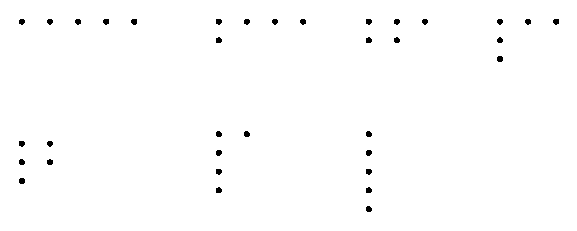
\includegraphics{yd}
\end{center}

The ``conjugate partition'' is obtained by taking the mirror image in
the main diagonal of the Young diagram.  (Or in other words, consider columns
instead of rows.)

By considering (conjugate) Young diagrams this theorem is immediate.

\begin{theorem}
The number of partions of $n$ into exactly $k$ parts equals the number of
partitions of $n$ with largest part $k$.
\end{theorem}

We now define an ordinary generating function for $p(n)$
\[
P(z) = 1 + \sum_{n \in \N} p(n) z^n.
\]

\begin{proposition}
\[
P(z) = \frac{1}{1-z} \frac{1}{1-z^2} \frac{1}{1-z^3} \dots
= \prod_{k \in \N} \frac{1}{1-z^k}.
\]
\end{proposition}

\begin{proof}
The RHS is
$(1 + z + z^2 + \dots) (1+ z^2 + z^4 + \dots) (1+ z^3 + z^6 \dots ) \dots$.

We get a term $z^n$ whenever we select $z^{a_1}$ from the first bracket,
$z^{2 a_2}$ from the second, $z^{3 a_3}$ from the third and so on, and
$n = a_1 + 2a_2 + 3 a_3 + \dots$, or in other words
$1^{a_1}\, 2^{a_2}\, 3^{a_3}\, \dots$ is a partition of $n$.  There are
$p(n)$ of these.
\end{proof}

We can similarly prove these results.

\begin{proposition}
The generating function $P_m(z)$ of the sequence $p_m(n)$ of partitions of
$n$ into at most $m$ parts (or the generating function for the sequence
$p_m(n)$ of partitions of $n$ with largest part $\le m$) satisfies
\[
P_m(z) = \frac{1}{1-z} \frac{1}{1-z^2} \frac{1}{1-z^3} \dots \frac{1}{1-z^m}.
\]
\end{proposition}

\begin{proposition}
The generating function for the number of partitions into odd parts is
\[
\frac{1}{1-z} \frac{1}{1-z^3} \frac{1}{1-z^5} \dots.
\]
\end{proposition}

\begin{proposition}
The generating function for the number of partitions into unequal parts is
\[
(1+z) (1+z^2) (1+z^3) \dots.
\]
\end{proposition}

\begin{theorem}
The number of partitions of $n$ into odd parts equals the number of
partitions of $n$ into unequal parts.
\end{theorem}

\begin{proof}
\begin{align*}
(1+z) (1+z^2) (1+z^3) \dots & = \frac{1-z^2}{1-z} \frac{1-z^4}{1-z^2}
\frac{1-z^6}{1-z^3} \dots \\
&= \frac{1}{1-z} \frac{1}{1-z^3} \frac{1}{1-z^5} \dots
\end{align*}
\end{proof}

\begin{theorem}
The number of self-conjugate partitions of $n$ equals the number of
partitions of $n$ into odd unequal parts.
\end{theorem}

\begin{proof}
Consider hooks along the main diagonal like this.

\begin{center}
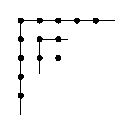
\includegraphics{self-conj}
\end{center}

This process can be reversed, so there is a one-to-one correspondance.
\end{proof}

\subsection{Generating function for self-conjugate partitions}

Observe that any self-conjugate partition consists of a largest
$k \times k$ subsquare and twice a partition of $\frac{1}{2}(n-k^2)$
into at most $k$ parts.  Now
\[
\frac{1}{(1-z^2) (1-z^4) \dots (1-z^{2m})}
\]
is the generating function for partitions of $n$ into even parts
of size at most $2 m$, or alternatively the generating function for partitions
of $\frac{1}{2} n$ into parts of size $\le m$.  We deduce that
\[
\frac{z^l}{(1-z^2) (1-z^4) \dots (1-z^{2m})}
\]
is the generating function for partitions of $\frac{1}{2}(n-l)$ into at most
$m$ parts.  Hence the generating function for self-conjugate partitions is
\[
1 + \sum_{k \in \N} \frac{z^{k^2}}{(1-z^2) (1-z^4) \dots (1-z^{2 k})}.
\]

Note also that this equals
\[
\prod_{k \in \N_0} (1+z^{2 k + 1}),
\]
as the number of self-conjugate partitions of $n$ equals the number of
partitions of $n$ into unequal odd parts.

In fact in any partition we can consider the largest $k \times k$ subsquare,
leaving two partitions of at most $k$ parts, one of $(n -k^2 - j)$, the
other of $j$ for some $j$.  The number of these two lots are the coefficients
of $z^{n - k^2 - j}$ and $z^j$ in $\prod_{i=1}^k \frac{1}{1-z^i}$
respectively.  Thus
\[
P(z) = 1 + \sum_{k \in \N} \frac{z^{k^2}}{\left(
(1-z) (1-z^2) \dots (1-z^k)\right)^2}.
\]

\chapter{Sets, Functions and Relations}

\section{Sets and indicator functions}

We fix some universal set $S$.  We write $P(S)$ for the set of all subsets
of $S$ --- the ``power set'' of $S$.  If $S$ is finite with
$\abs{S} = m$ (the number of elements), then $\abs{P(S)} = 2^m$.

Given a subset $A$ of $S$ ($A \subseteq S$) we define the ``complement''
$\Bar{A}$ of $A$ in $S$ as $\Bar{A} = \{ s \in S : s \notin A \}$.

Given two subsets $A$, $B$ of $S$ we can define various operations to get
new subsets of $S$.
\begin{align*}
A \cap B &= \{ s \in S : s \in A \text{ and } s \in B \} \\
A \cup B &= \{ s \in S : s \in A \text{ (inclusive) or } s \in B \} \\
A \setminus B &= \{ s \in A : s \notin B \} \\
A \circ B & = \{s \in S : s \in A \text{ (exclusive) or } s \in B \}
& & \text{the symmetric difference} \\
&= (A \cup B) \setminus (A \cap B) \\
&= (A \setminus B) \cup (B \setminus A).
\end{align*}

The indicator function $I_A$ of the subset $A$ of $S$ is the function
$I_A \colon S \mapsto \{0,1\}$ defined by
\[
I_A(s) = \begin{cases}
1 & x \in A \\
0 & \text{otherwise.}
\end{cases}
\]
It is also known as the characteristic function $\chi_A$.  Two subsets
$A$ and $B$ of $S$ are equal iff $I_A(s) = I_B(s)\ \forall s \in S$.  These
relations are fairly obvious:

\begin{align*}
I_{\Bar{A}} &= 1 - I_A \\
I_{A \cap B} &= I_A \cdot I_B \\
I_{A \cup B} &= I_A + I_B \\
I_{A \circ B} &= I_A + I_B \mod{2}.
\end{align*}

\begin{proposition}
$A \circ (B \circ C) = (A \circ B) \circ C$.
\end{proposition}

\begin{proof}
For, modulo 2, 
\[
I_{A \circ (B \circ C)} = I_A + I_{B \circ C}
= I_A + I_B + I_C = I_{A \circ B} + I_C = I_{(A \circ B) \circ C} \mod{2}.
\]
\end{proof}

Thus $P(S)$ is a group under $\circ$.  Checking the group axioms we get:

\begin{itemize}
\item Given $A, B \in P(S)$, $A \circ B \in P(S)$ ---  closure,
\item $A \circ (B \circ C) = (A \circ B) \circ C$ --- associativity,
\item $A \circ \emptyset = A$ for all $A \in P(S)$ --- identity,
\item $A \circ A = \emptyset$ for all $A \in P(S)$ --- inverse.
\end{itemize}

We note that $A \circ B = B \circ A$ so that this group is abelian.

\subsection{De Morgan's Laws}

\begin{proposition}
\begin{enumerate}
\item $\overline{A \cap B} = \Bar{A} \cup \Bar{B}$
\item $\overline{A \cup B} = \Bar{A} \cap \Bar{B}$
\end{enumerate}
\end{proposition}

\begin{proof}
\begin{align*}
I_{\overline{A \cap B}} &= 1- I_{A \cap B} = 1 - I_A I_B \\
&= (1-I_A) + (1-I_B) - (1-I_A)(1-I_B) \\
&= I_{\Bar{A}} + I_{\Bar{B}} - I_{\Bar{A} \cap \Bar{B}} \\
&= I_{\Bar{A} \cup \Bar{B}}.
\end{align*}

We prove $2$ by using $1$ on $\Bar{A}$ and $\Bar{B}$.
\end{proof}

A more general version of this is:  Suppose $A_1, \dots, A_n \subseteq S$.
Then
\begin{enumerate}
\item $\overline{\bigcap_{i=1}^n A_i} = \bigcup_{i=1}^n \Bar{A_i}$
\item $\overline{\bigcup_{i=1}^n A_i} = \bigcap_{i=1}^n \Bar{A_i}$.
\end{enumerate}
These can be proved by induction on $n$.


\subsection{Inclusion-Exclusion Principle}

Note that $\abs{A} = \sum_{s \in S} I_A(s)$.

\begin{theorem}[Principle of Inclusion-Exclusion]\label{T:PIE}
Given $A_1, \dots, A_n \subseteq S$ then
\[
\abs{A_1 \cup \dots \cup A_n} = \sum_{\emptyset \neq J \subseteq \{1,\dots,n\}}
(-1)^{\abs{J} - 1} \abs{A_J}, \text{where $A_J = \bigcap_{i \in J} A_i$.} 
\]
\end{theorem}

\begin{proof}
We consider $\overline{A_1 \cup \dots \cup A_n}$ and note that
\begin{align*}
I_{\overline{A_1 \cup \dots \cup A_n}} &= I_{\Bar{A_1} \cap \dots \cap
\Bar{A_n}} \\
&= I_{\Bar{A_1}} I_{\Bar{A_2}} \dots I_{\Bar{A_n}} \\
&= (1-I_{A_1}) (1 - I_{A_2}) \dots (1 - I_{A_n}) \\
&= \sum_{J \subseteq \{ 1, \dots, n \}} (-1)^{\abs{J}} I_{A_J},
\end{align*}

Summing over $s \in S$ we obtain the result
\[
\abs{\overline{A_1 \cup \dots \cup A_n}} = \sum_{J \subseteq
\{ 1, \dots, n \}} (-1)^{\abs{J}} \abs{A_J},
\]
which is equivalent to the required result.
\end{proof}

Just for the sake of it, we'll prove it again!

\begin{proof}
For each $s \in S$ we calculate the contribution.  If $s \in S$ but
$s$ is in no $A_i$ then there is a contribution $1$ to the left.  The
only contribution to the right is $+1$ when $J = \emptyset$.  If
$s \in S$ and $K = \{ i \in \{1, \dots, n \} : s \in A_i \}$ is non-empty
then the contribution to the right is $\sum_{I \subseteq K}
(-1)^{\abs{I}} = \sum_{i=0}^k \binom{k}{i} (-1)^i = 0$, the same as
on the left.
\end{proof}

\begin{example}[Euler's Phi Function]
\[
\phi(m) = m \prod_{\substack{p \text{ prime} \\ p \mid m}} \left(1-\frac{1}{p}
\right).
\]
\end{example}

\begin{proof}[Solution]
Let $m = \prod_{i=1}^n p_i^{a_i}$, where the $p_i$ are distinct primes
and $a_i \in \N$.  Let $A_i$ be the set of integers less than $m$ which
are divisible by $p_i$.  Hence $\phi(m) = \abs{\bigcap_{i=1}^n \Bar{A_i}}$.
Now $\abs{A_i} = \frac{m}{p_i}$, in fact for $J \subseteq \{ 1, \dots, m \}$
we have $\abs{A_J} = \frac{m}{\prod_{i \in J} p_i}$.  Thus
\begin{align*}
\phi(m) & = m - \frac{m}{p_1} - \frac{m}{p_2} - \dots -
\frac{m}{p_n} \\
&+ \frac{m}{p_1 p_2} + \frac{m}{p_1 p_3} + \dots + \frac{m}{p_2 p_3}
+ \dots + \frac{m}{p_{n-1} p_n} \\
&\vdots \\
&+ (-1)^n \frac{m}{p_1 p_2 \dots p_n} \\
& = m \prod_{\substack{p \text{ prime} \\ p \mid m}} \left(1-\frac{1}{p}
\right) \qquad \text{as required.}
\end{align*}
\end{proof}

\begin{example}[Derangements]
Suppose we have $n$ psychologists at a meeting.
Leaving the meeting they pick up their overcoats at random.  In how many
ways can this be done so that none of them has his own overcoat.  This
number is $D_n$, the number of derangements of $n$ objects.
\end{example}

\begin{proof}[Solution]
Let $A_i$ be the number of ways in which psychologist $i$ collects his own
coat.  Then $D_n = \abs{\Bar{A_1} \cap \dots \cap \Bar{A_n}}$.
If $J \subseteq \{1, \dots, n \}$ with $\abs{J} = k$ then
$\abs{A_J} = (n-k)!$.  Thus
\begin{align*}
\abs{\Bar{A_1} \cap \dots \cap \Bar{A_n}} &= n! - \binom{n}{1} (n-1)!
+ \binom{n}{2} (n-2)! - \dots \\
&= n! \sum_{k=0}^n \frac{(-1)^k}{k!}.
\end{align*}

Thus $D_n$ is the nearest integer to $n!\, e^{-1}$, since $\frac{D_n}{n!}
\to e^{-1}$ as $n \to \infty$.
\end{proof}

\section{Functions}

Let $A,B$ be sets.  A function (or mapping, or map) $f \colon A \mapsto B$
is a way to associate a unique image $f(a) \in B$ with each $a \in A$.  If
$A$ and $B$ are finite with $\abs{A} = m$ and $\abs{B} = n$ then the
set of all functions from $A$ to $B$ is finite with $n^m$ elements.

\begin{definition}
The function $f \colon A \mapsto B$ is injective (or one-to-one) if
$f(a_1) = f(a_2)$ implies that $a_1 = a_2$ for all $a_1, a_2 \in A$.
\end{definition}

The number of injective functions from an $m$-set to an $n$-set is
$n^{\underline{m}}$.

\begin{definition}
The function $f \colon A \mapsto B$ is surjective (or onto) if each
$b \in B$ has at least one preimage $a \in A$.
\end{definition}

The number of surjective functions from an $m$-set to an $n$-set is
$n!\, S(m,n)$.

\begin{definition}
The function $f \colon A \mapsto B$ is bijective if it is both injective
and surjective.
\end{definition}

If $A$ and $B$ are finite then $f \colon A \mapsto B$ can only be bijective
if $\abs{A} = \abs{B}$.  If $\abs{A} = \abs{B} < \infty$ then any
injection is a bijection; similarly any surjection is a bijection.  There
are $n!$ bijections between two $n$-sets.

If $A$ and $B$ are infinite then there exist injections which are not
bijections and \emph{vice versa}.  For instance if $A = B = \N$, define
\[
f(n) = \begin{cases}
1 & n = 1 \\
n-1 & \text{otherwise}
\end{cases} \qquad \text{and} \qquad
g(n) = n+1.
\]

Then $f$ is surjective but not injective and $g$ is injective but
not surjective.

\begin{proposition}
\[
n!\, S(m,n) = \sum_{k=0}^n (-1)^k \binom{n}{k} (n-k)^m
\]
\end{proposition}

\begin{proof}
This is another application of the Inclusion-Exclusion principle.  Consider
the set of functions from $A$ to $B$ with $\abs{A} = m$ and
$\abs{B} = n$. For any $i \in B$, define $X_i$ to be the set of functions
avoiding $i$.

So the set of surjections is $\Bar{X_1} \cap \dots \cap \Bar{X_n}$.
Thus the number of surjections from $A$ to $B$ is
$\abs{\Bar{X_1} \cap \dots \cap \Bar{X_n}}$.  By the inclusion-exclusion
principle this is $\sum_{J \subseteq B} (-1)^{\abs{J}} \abs{X_J}$.
If $\abs{J} = k$ then $\abs{X_J} = (n-k)^m$.  The result follows.
\end{proof}

Mappings can be ``composed''.  Given $f \colon A \mapsto B$ and
$g \colon B \mapsto C$ we can define $gf \colon A \mapsto C$ by
$gf(a) = g(f(a))$.  If $f$ and $g$ are injective then so is $gf$, similarly
for surjectivity.  If we also have $h \colon C \mapsto D$, then associativity
of composition is easily verified : $(hg)f \equiv h(gf)$.

\section{Permutations}

A permutation of $A$ is a bijection $f \colon A \mapsto A$.  One notation
is
\[
f = \begin{pmatrix}
1 & 2 & 3 & 4 & 5 & 6 & 7 & 8 \\
1 & 3 & 4 & 2 & 8 & 7 & 6 & 5
\end{pmatrix}.
\]

The set of permutations of $A$ is a group under composition, the symmetric
group $\sym A$.  If $\abs{A} = n$ then $\sym A$ is also denoted $S_n$ and
$\abs{\sym A} = n!$.  $S_n$ is not abelian --- you can come up with
a counterexample yourself. We can also think of permutations
as directed graphs, in which case the following becomes clear.

\begin{proposition}
Any permutation is the product of disjoint cycles.
\end{proposition}

We have a new notation for permutations, cycle notation.%
\footnote{See the Algebra and Geometry course for more details.}  For our
function $f$ above, we write
\[
f = (1) (2\ 3\ 4) (5\ 8) (6\ 7) = (2\ 3\ 4) (5\ 8) (6\ 7).
\]

\subsection{Stirling numbers of the first kind}

\begin{definition}
$s(n,k)$ is the number of permutations of $\{1,\dots,n\}$ with precisely
$k$ cycles (including fixed points).
\end{definition}

For instance $s(n,n) = 1$, $s(n,n-1) = \binom{n}{2}$, $s(n,1) = (n-1)!$,
$s(n,0) = s(0,k) = 0$ for all $k,n \in \N$ but $s(0,0) = 1$.

\begin{lemma}
\[
s(n,k) = s(n-1,k-1) + (n-1) s(n-1,k)
\]
\end{lemma}

\begin{proof}
Either the point $n$ is in a cycle on its own ($s(n-1,k-1)$ such) or it
is not.  In this case, $n$ can be inserted into any of $n-1$ places in
any of the $s(n-1,k)$ permutations of $\{1,\dots,n-1 \}$.
\end{proof}

We can use this recurrence to prove this proposition. (Proof left as exercise.)

\begin{proposition}
\[
x^{\overline{n}} = \sum_k s(n,k) x^k
\]
\end{proposition}

\subsection{Transpositions and shuffles}

A transposition is a permutation which swaps two points and fixes the rest.

\begin{theorem}
Every permutation is the product of transpositions.
\end{theorem}

\begin{proof}
Since every permutations is the product of cycles we only need to check
for cycles.  This is easy: $(i_1\ i_2\ \dots\ i_k) = (i_1\ i_2)
(i_2\ i_3) \dots (i_{k-1}\ i_k)$.
\end{proof}

\begin{theorem}\label{T:permsign}
For a given permutation $\pi$, the number of transpositions used to
write $\pi$ as their product is either always even or always odd.
\end{theorem}

We write $\sign \pi = \begin{cases}
+1 & \text{if always even}\\
-1 & \text{if always odd}
\end{cases}$.  We say that $\pi$ is an \begin{tabular}{c} even \\ odd
\end{tabular} permutation.

Let $c(\pi)$ be the number of cycles in the disjoint cycle representation
of $\pi$ (including fixed points).

\begin{lemma}
If $\sigma = (a\ b)$ is a transposition that $c(\pi \sigma) = c(\pi) \pm 1$.
\end{lemma}

\begin{proof}
If $a$ and $b$ are in the same cycle of $\pi$ then $\pi \sigma$ has two
cycles, so $c(\pi \sigma) = c(\pi) + 1$.  If $a$ and $b$ are in different
cycles then they contract them together and $c(\pi \sigma) = c(\pi) - 1$.
\end{proof}

\begin{proof}[Proof of theorem \ref{T:permsign}]
Assume $\pi = \sigma_1 \dots \sigma_k \iota = \tau_1 \dots \tau_l \iota$.  Then
$c(\pi) = c(\iota) + k \equiv c(\iota) + l \pmod{2}$.  Hence $k \equiv
l \pmod{2}$ as required.
\end{proof}

We note that $\sign \pi = (-1)^{n - c(\pi)}$, thus $\sign (\pi_1 \pi_2)
= \sign \pi_1 \sign \pi_2$ and thus $\sign$ is a homomorphism from
$S_n$ to $\{ \pm 1 \}$.

A $k$-cycle is an even permutation iff $k$ is odd.  A permutation is
an \begin{tabular}{c} even \\ odd \end{tabular} permutation iff the number
of even length cycles in the disjoint cycle representation is
\begin{tabular}{c} even \\ odd \end{tabular}.

\subsection{Order of a permutation}

If $\pi$ is a permutation then the order of $\pi$ is the least natural
number $n$ such that $\pi^n = \iota$.  The order of the permutation $\pi$
is the lcm of the lengths of the cycles in the disjoint cycle decomposition
of $\pi$.

In card shuffling we need to maximise the order of the relevant permutation
$\pi$.  One can show (see) that for $\pi$ of maximal length we can take
all the cycles in the disjoint cycle representation to have prime power length.
For instance with $30$ cards we can get a $\pi \in S_{30}$ with an order of
$4620$ (cycle type $3\ 4\ 5\ 7\ 11$).

\subsection{Conjugacy classes in $S_n$}

Two permutations $\alpha, \beta \in S_n$ are conjugate iff $\exists \pi
\in S_n$ such that $\alpha = \pi \beta \pi^{-1}$.

\begin{theorem}
Two permutations are conjugate iff they have the same cycle type.
\end{theorem}

This theorem is proved in the Algebra and Geometry course.  We note the
corollary that the number of conjugacy classes in $S_n$ equals the number
of partitions of $n$.

\subsection{Determinants of an $n \times n$ matrix}

In the Linear Maths course you will prove that if $A = (a_{ij})$ is an
$n \times n$ matrix then
\[
\det A = \sum_{\pi \in S_n} \sign \pi \prod_{j=1}^n a_{j\, \pi(j)}.
\]

\section{Binary Relations}

A binary relation on a set $S$ is a property that any pair of elements
of $S$ may or may not have.  More precisely:

Write $S \times S$, the Cartesian square of $S$ for the set of pairs
of elements of $S$, $S \times S = \{ (a,b) : a,b \in S \}$.  A binary
relation $\relset$ on $S$ is a subset of $S \times S$.  We write $a \rel b$
iff $(a,b) \in \relset$.  We can think of $\relset$ as a directed graph
with an edge from $a$ to $b$ iff $a \rel b$.

A relation $\relset$ is:

\begin{itemize}
\item reflexive iff $a \rel a\ \forall a \in S$,
\item symmetric iff $a \rel b \Rightarrow b \rel a\ \forall a,b \in S$,
\item transitive iff $a \rel b, b \rel c \Rightarrow a \rel c\ \forall
a,b,c \in S$,
\item antisymmetric iff $a \rel b, b \rel a \Rightarrow a = b\ \forall
a,b \in S$.
\end{itemize}

The relation $\relset$ on $S$ is an equivalence relation if it is reflexive,
symmetric and transitive.  These are ``nice'' properties designed to make
$\relset$ behave something like $=$.

\begin{definition}
If $\relset$ is a relation on $S$, then
\[
[a]_\relset = [a] = \{ b \in S : a \rel b \}.
\]
\end{definition}

If $\relset$ is an equivalence then these are the equivalence classes.

\begin{theorem}
If $\relset$ is an equivalence relation then the equivalence classes
form a partition of $S$.
\end{theorem}

\begin{proof}
If $a \in S$ then $a \in [a]$, so the classes cover all of $S$.  If
$[a] \cap [b] \neq \emptyset$ then $\exists c \in [a] \cap [b]$.  Now
$a \rel c$ and $b \rel c \Rightarrow c \rel b$.  Thus $a \rel b$ and
$b \in [a]$.  If $d \in [b]$ then $b \rel d$ so $a \rel d$ and thus
$[b] \subseteq [a]$.  We can similarly show that $[a] \subseteq [b]$
and thus $[a] = [b]$.
\end{proof}

The converse of this is true: if we have a partition of $S$ we can
define an equivalence relation on $S$ by $a \rel b$ iff $a$ and $b$ are in
the same part.

An application of this is the proof of Lagrange's Theorem.  The idea
is to show that being in the same (left/right) coset is an equivalence
relation.

Given an equivalence class on $S$ the quotient set is $S/\relset$, the
set of all equivalence classes.  For instance if $S=\R$ and
$a \rel b$ iff $a - b \in \Z$ then $S/\relset$ is (topologically) a circle.
If $S = \R^2$ and $(a_1,b_1) \rel (a_2,b_2)$ iff $a_1 - a_2 \in \Z$ and
$b_1 - b_2 \in \Z$ the quotient set is a torus.

Returning to a general relation $\relset$, for each $k \in \N$ we define
\[
\relset^{(k)} = \{ (a,b) : \text{there is a path of length at $k$ from
$a$ to $b$} \}.
\]

$\relset^{(1)} = \relset$ and $\relset^{(\infty)} = t(R)$, the transitive
closure of $\relset$.  $\relset^{(\infty)}$ is defined as
$\bigcup_{i \ge 1} \relset^{(i)}$.

\section{Posets}

$\relset$ is a (partial) order on $S$ if it is reflexive, anti-symmetric
and transitive.  The set $S$ is a poset (partially ordered set) if there
is an order $\relset$ on $S$.

We generally write $a \le b$ iff $(a,b) \in \relset$, and $a < b$ iff
$a \le b$ and $a \neq b$.

Consider $D_n$, the set of divisors of $n$.  $D_n$ is partially ordered
by division, $a \le b$ if $a \mid b$.  We have the Hasse diagram, in this
case for $D_{36}$:

\begin{center}
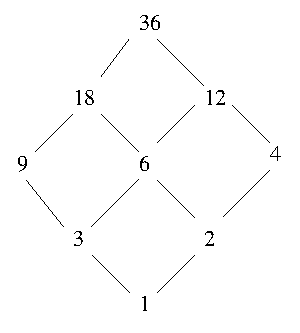
\includegraphics{hasse}
\end{center}

A descending chain is a sequence $a_1 > a_2 > a_3 > \dots$.  An
antichain is a subset of $S$ with no two elements directly comparable,
for instance $\{4,6,9\}$ in $D_{36}$.

\begin{proposition}
If $S$ is a poset with no chains of length $> n$ then $S$ can be covered
by at most $n$ antichains.
\end{proposition}

\begin{proof}
Induction on $n$.  Take $n > 1$ and let $M$ be the set of all maximal elements
in $S$.  Now $S \setminus M$ has no chains of length $> n - 1$ and $M$
is an antichain.
\end{proof}

\subsection{Products of posets}

Suppose $A$ and $B$ are posets.  Then $A \times B$ has various orders;
two of them being
\begin{itemize}
\item product order: $(a_1,b_1) \le (a_2,b_2)$ iff $a_1 \le a_2$
and $b_1 \le b_2$,
\item lexicographic order:  $(a_1,b_1) \le (a_2,b_2)$ if either
$a_1 \le a_2$ or if $a_1 = a_2$ then $b_1 \le b_2$.
\end{itemize}

Exercise: check that these are orders.

Note that there are no infinite descending chains in $\N \times \N$
under lexicographic order.  Such posets are said to be well ordered.  The
principle of induction follows from well-ordering as discussed earlier.

\subsection{Eulerian Digraphs}

A digraph is Eulerian if there is a closed path covering all the edges.
A necessary condition is: the graph is connected and even (each vertex
has an equal number of ``in'' and ``out'' edges).  This is in fact sufficient.

\begin{proposition}
The set of such digraphs is well-ordered under containment.
\end{proposition}

\begin{proof}
Assume proposition is false and let $G$ be a minimal counterexample.  Let
$T$ be a non-trivial closed path in $G$, for instance the longest closed path.
Now $T$ must be even, so $G \setminus T$ is even.  Hence each connected
component of $G \setminus T$ is Eulerian as $G$ is minimal.  But then $G$
is Eulerian: you can walk along $T$ and include all edges of connected
components of $G \setminus T$ when encountered --- giving a contradiction.
Hence there are no minimal counterexamples.
\end{proof}

\section{Countability}

\begin{definition}
A set $S$ is countable if either $\abs{S} < \infty$ or $\exists$ a bijection
$f \colon S \mapsto \N$.
\end{definition}

The countable sets can be equivalently thought of as those that can be listed
on a line.

\begin{lemma}
Any subset $S \subset \N$ is countable.
\end{lemma}

\begin{proof}
For: map the smallest element of $S$ to $1$, the next smallest to $2$
and so on.
\end{proof}

\begin{lemma}
A set $S$ is countable iff $\exists$ an injection $f \colon S \mapsto \N$.
\end{lemma}

\begin{proof}
This is clear for finite $S$.  Hence assume $S$ is infinite.  If $f \colon
S \mapsto \N$ is an injection then $f(S)$ is an infinite subset of $\N$.
Hence $\exists$ a bijection $g \colon f(S) \mapsto \N$. Thus
$gf \colon S \mapsto \N$ is a bijection.
\end{proof}

An obvious result is that if $S'$ is countable and $\exists$ an injection
$f \colon S \mapsto S'$ then $S$ is countable.

\begin{proposition}
$\Z$ is countable.
\end{proposition}

\begin{proof}
Consider $f \colon \Z \mapsto \N$,
\[
f \colon x \mapsto \begin{cases}
2 x + 1 & \text{if $x \ge  0$} \\
- 2 x & \text{if $x < 0$.} 
\end{cases}
\]

This is clearly a bijection.
\end{proof}

\begin{proposition}
$\N^k$ is countable for $k \in \N$.
\end{proposition}

\begin{proof}
The map $(i_1, \dots, i_k) \mapsto 2^{i_1} 3^{i_2} \dots p_k^{i_k}$
($p_j$ is the $j^{\text{th}}$ prime) is an injection by uniqueness of prime
factorisation.
\end{proof}

\begin{lemma}
If $A_1, \dots, A_k$ are countable with $k \in \N$, then so is
$A_1 \times \dots \times A_k$.
\end{lemma}

\begin{proof}
Since $A_i$ is countable there exists an injection $f_i \colon A_i \mapsto \N$.
Hence the function $g \colon A_1, \dots, A_k \mapsto \N^k$ defined by
$g(a_1,\dots,a_k) = (f_1(a_1),\dots,f_k(a_k))$ is an injection.
\end{proof}

\begin{proposition}
$\Q$ is countable.
\end{proposition}

\begin{proof}
Define $f \colon \Q \mapsto \N$ by
\[
f \colon \frac{a}{b} \mapsto 2^{\abs{a}} 3^b 5^{1+\sign a},
\]
where $(a,b) = 1$ and $b > 0$.
\end{proof}

\begin{theorem}
A countable union of countable sets is countable.  That is, if $I$ is a
countable indexing set and $A_i$ is countable $\forall i \in I$ then
$\bigcup_{i \in I} A_i$ is countable.
\end{theorem}

\begin{proof}
Identify first $I$ with the subset $f(I) \subseteq \N$.
Define $F \colon A \mapsto \N$ by $ a \mapsto 2^n 3^m$ where
$n$ is the smallest index $i$ with $a \in A_i$, and $m = f_n(a)$.  This
is well-defined and injective (stop to think about it for a bit).
\end{proof}

\begin{theorem}
The set of all algebraic numbers is countable.
\end{theorem}

\begin{proof}
Let $P_n$ be the set of all polynomials of degree at most $n$ with integral
coefficients.  Then the map $c_n x^n + \dots + c_1 x + c_0
\mapsto (c_n, \dots, c_1, c_0)$ is an injection from $P_n$ to $\Z^{n+1}$.
Hence each $P_n$ is countable.  It follows that the set of all polynomials
with integral coefficients is countable.  Each polynomial has finitely
many roots, so the set of algebraic numbers is countable.
\end{proof}

\begin{theorem}[Cantor's diagonal argument]
$\R$ is uncountable.
\end{theorem}

\begin{proof}
Assume $\R$ is countable, then the elements can be listed as
\begin{align*}
r_1 &= n_1 . d_{11} d_{12} d_{13} \dots \\
r_2 &= n_2 . d_{21} d_{22} d_{13} \dots \\
r_3 &= n_3 . d_{31} d_{32} d_{33} \dots
\end{align*}
(in decimal notation).  Now define the real
$r = 0.d_1 d_2 d_3 \dots$ by $d_i = 0$ if $d_{ii} \neq 0$ and $d_i
= 1$ if $d_{ii} = 0$.  This is real, but it differs from $r_i$ in the
$i^{\text{th}}$ decimal place.  So the list is incomplete and the
reals are uncountable.
\end{proof}

Exercise: use a similiar proof to show that $P(\N)$ is uncountable.

\begin{theorem}
The set of all transcendental numbers is uncountable.  (And therefore
at least non-empty!)
\end{theorem}

\begin{proof}
Let $A$ be the set of algebraic numbers and $T$ the set of transcendentals.
Then $\R = A \cup T$, so if $T$ was countable then so would $\R$ be.  Thus
$T$ is uncountable.
\end{proof}

\section{Bigger sets}

The material from now on is starred.

Two sets $S$ and $T$ have the same \emph{cardinality}  ($\abs{S}
= \abs{T}$) if there is a bijection between $S$ and $T$. One can show
(the Schr\"oder-Bernstein theorem) that if there is an injection from
$S$ to $T$ and an injection from $T$ to $S$ then there is a bijection
between $S$ and $T$.

For any set $S$, there is an injection from $S$ to $P(S)$, simply
$x \mapsto \{ x \}$.  However there is never a surjection $S
\mapsto P(S)$, so $\abs{S} < \abs{P(S)}$, and so
\[
\abs{\N} < \abs{P(\N)} < \abs{P(P(\N))} < \dots
\]
for some sensible meaning of $<$.

\begin{theorem}
There is no surjection $S \mapsto P(S)$.
\end{theorem}

\begin{proof}
Let $f \colon S \mapsto P(S)$ be a surjection and consider
$X \in P(S)$ defined by $ \{ x \in S : x \notin f(x) \}$.  Now
$\exists x' \in S$ such that $f(x') = X$.  If $x' \in X$ then
$x' \notin f(x')$ but $f(x') = X$ --- a contradiction.  But if $x' \notin
X$ then $x' \notin f(x')$ and $x' \in X$ --- giving a contradiction either
way. 
\end{proof}

If there is an \begin{tabular}{c} injection
\\ surjection \end{tabular} $f \colon A \mapsto B$ then there exists
a \begin{tabular}{c} surjection
\\ injection \end{tabular} $g \colon B \mapsto A$.  Moreover we
can ensure that \begin{tabular}{c} $g \circ f = \iota_A$
\\ $f \circ g = \iota_B$ \end{tabular} 

\backmatter

\begin{thebibliography}{9}

\bibitem{Hardy} Hardy \& Wright, \emph{An Introduction to the Theory
    of Numbers}, Fifth ed., OUP, 1988.
  
  {\sffamily \small This book is relevant to quite a bit of the
    course, and I quite enjoyed (parts of!) it. }
  
\bibitem{Davenport} H. Davenport, \emph{The Higher Arithmetic}, Sixth
  ed., CUP, 1992.
  
  {\sffamily \small A \emph{very} good book for this course.  It's
    also worth a read just for interest's sake. }

\end{thebibliography}

I've also heard good things about Biggs' book, but haven't read
it.

\end{document}
